\section{Pairwise Sublinear Additive Spanners}
\label{sec: pairwise}

In this section, we prove the following \Cref{pairwise-sublinear}, which will serve as a building block for \Cref{sublinear}. 
%In the algorithm for \Cref{pairwise-sublinear}, we design a subroutine called \pathpart, which will also be used in our sub-quadratic time algorithm for \Cref{subquad}.
Throughout this section, we use the following stretch function $f$: for any parameter $\epsilon > 0$ and any integer $k\geq 1$, $f_{k, \epsilon}(d) = d + 2^{30k/\epsilon}d^{1-1/k}$.
%This section is devoted to the following statement.

\begin{lemma}\label{pairwise-sublinear}
For any undirected unweighted graph $G = (V, E)$ on $n$ vertices, any collection $\pset\subseteq V\times V$ of pairs of its vertices, any integer $k\geq 1$ and parameter $0<\epsilon<1$, there is a subgraph $H\subseteq G$ with $O(2^{2k/\epsilon}n^{1+10k\epsilon}|\pset|^{1 / 2^{k+1}})$ edges, such that for every pair $(s, t)\in \pset$, $\dist_H(s, t)\leq f_{k, \epsilon}(\dist_G(s, t))$.
\end{lemma}

\subsection{Preparation and a subrountine}

We prove \Cref{pairwise-sublinear} by an induction on $k$. The base case (when $k=1$) immediately follows from \Cref{pairwise-spanner}. We assume now that \Cref{pairwise-sublinear} is correct for $1,\ldots, k-1$.
We will design an algorithm that computes a pairwise additive spanner required in \Cref{pairwise-sublinear}. At a high level, our algorithm can be viewed as a combination of the clustering algorithm (\Cref{clustering}) from \cite{bodwin2021better} and the path-buying schemes from \cite{kavitha2017new}. 

%As the basis, when $k = 1$, we can directly apply Lemma \ref{pairwise-spanner}. For the rest we assume $k>1$, and that the statement holds for $k-1$.

%\paragraph{Preparation.} 
For each integer $D\in \set{1,2,2^2,\ldots,2^{\floor{\log n}}}$, we will construct a subgraph $H_D\subseteq G$, such that for all pairs $(s,t)\in \pset$ with $D\le \dist_G(s, t) <2D$, $\dist_{H_D}(s, t)\leq \dist_G(s, t) + 2^{30k/\epsilon}D^{1-1/k}$ holds.
%If it is possible, then we can take the union of the spanners ranging over all different choices of $D$ to finish the inductive step.
We will then let $H=\bigcup_{0\le i\le \floor{\log n}}H_{2^i}$ to finish the construction.


%Without loss of generality, assume $D^{1-1/k}$ is an integer. 
We now describe the construction of the subgraph $H_D$.
We first apply the algorithm from Lemma \ref{clustering} to graph $G$ with parameters $R=D^{1-1/k}$ and $\epsilon$; for convenience, we will assume $D^{1-1/k}$ is an integer. Let $\clusters$ be the collection of balls we get.
%For each ball $\ball(c, r)\in\clusters$, let $T_c$ be a BFS tree that is rooted at $c$ and spans all vertices in $\ball(c, 4r)$. 
We will also iteratively construct, for each ball $\ball(c,r)\in \balls$, a set $\pset_c\subseteq \ball(c, 4r)\times\ball(c, 4r)$ of pairs, which is initially empty.
Over the course of the algorithm, we maintain the graph $H_D$ as the union of the following edges over all balls $\ball(c, r)\in \clusters$:
\begin{enumerate}[(i)]
	\item a BFS tree $T_c$ that is rooted at $c$ and spans all vertices in $G[\ball(c, 4r)]$;
	\item a pairwise spanner of $G[\ball(c, 4r)]$ with respect to the set $\pset_c$ of pairs, with stretch function $f_{k-1, \epsilon}$ and size $O(2^{2k/\epsilon}|\ball(c, 4r)|^{1+10k\epsilon} |\pset_c|^{1 / 2^{k+1}})$, whose existence is guaranteed by the inductive hypothesis. %(that \Cref{pairwise-sublinear} is true for $k-1$).
	When the sets $\set{\pset_c}$ change during our construction algorithm, the graph $H_D$ evolves with them.
\end{enumerate}


\iffalse
 refers to the spanner under construction, which is updated from time to time as demand pairs $P_c$ are changing throughout the course. At any moment during the execution of the algorithm, the spanner $H$ is defined as the union of the following two types of edges.
\begin{framed}
	Construction of spanner $H$
	\begin{itemize}
		\item For each $\ball(c, r)\in\clusters$, construct an arbitrary breath-first search tree rooted at $c$ that spans $\ball(c, 4r)$ in $G$.
		\item For each $\ball(c, r)\in \clusters$, inductively build a pairwise spanner on demand pairs $P_c$ in $G[\ball(c, 4r)]$ with sublinear stretch function $f_{k-1, \epsilon}(\cdot)$.
	\end{itemize}
\end{framed}
\fi


In order to construct the sets $\set{\pset_c}$, we will take a path-buying approach. Specifically, we will iteratively find a short path that contains relatively few new edges and ``settles'' many pairs of clusters (by connecting them in a near-optimal way). As the construction of $H_D$ is recursive, we will distribute the task of ``buying this path'' to the clusters in $\bset$ as in \cite{bodwin2021better}, which requires us to first chop up a shortest path into short segments. For this, we need the following subroutine called $\pathpart$, which was initially proposed in \cite{bodwin2021better}.

\paragraph{Subroutine \pathpart.} The input to subrountine \pathpart is a shortest path $\pi$ connecting a pair $s,t$ of vertices in a graph $G$ and a collection $\balls$ of balls that covers all vertices in $G$, and the output is a partitioning of path $\pi$ as the sequential concatenation of its subpaths $\pi = \alpha_1\circ\alpha_2\circ\cdots \circ\alpha_l$, such that, for each $1\le i\le l$, if we denote by $s_i, t_i$ the endpoints of $\alpha_i$ (so $\alpha_i=\pi[s_i,t_i]$), then there exists a ball $\ball(c_i, r_i)\in \clusters$, such that $s_i\in \ball(c_i, r_i)$ and $t_i\in \ball(c_i, 2r_i)$, and we say that the ball $\ball(c_i, r_i)$ \emph{hosts} the subpath $\alpha_i$.

%To determine all the sub-paths and balls $\alpha_i, \ball(c_i, r_i), 1\leq i\leq l$, we will use a variable vertex $v\leftarrow s$ on $\pi$ that moves from $s$ to $t$ iteratively. In each iteration, if $v$ has not reached the other endpoint $t$, namely $v\neq t$, by the coverage property we can always find a ball $\ball(c, r)\in\clusters$ such that $v\in \ball(c, r)$. Then, let $w\in \pi(v, t]\cap \ball(c, 2r)$ be the vertex which is closest to $t$. Assign $\alpha_i\leftarrow \pi[v, w]$ and $\ball(c_i, r_i)\leftarrow \ball(c, r)$, and increment $i\leftarrow i+1$ and update $v\leftarrow w$. When the above iterative procedure terminates, we end up with a sequence of sub-paths $\alpha_1, \alpha_2, \cdots, \alpha_l$ and balls $\ball(c_1, r_{c_1}), \ball(c_2, r_{c_2}), \cdots, \ball(c_l, r_{c_l})$. 

We start by directing $\pi$ from $s$ to $t$ and setting $s_1=s$. Since $s_1$ is covered by $\balls$, there exists a ball in $\bset$ that contains $s_1$, and we designate this ball as $\ball(c_1,r_{1})$. We then find the \textbf{last} vertex on $\pi$ that lies in $\ball(c_1,2r_{1})$, and designate it as $t_1$. The first subpath is then defined to be $\alpha_1=\pi[s_1,t_1]$. We then set $s_2=t_1$ and repeat the process to find subpaths $\alpha_2,\ldots,\alpha_l$ until all edges are included in some subpath; that is, for a general index $i\geq 2$, if $s_i\neq t$, then find a ball $\ball(c_i, r_i)\in\bset$ containing $s_i$, and define $t_i\in \pi(s_i, t]\cap \ball(c_i, 2r_i)$ to be the vertex on $\pi$ which is closest to $t$. After that, if $t_i\neq t$, assign $s_{i+1} = t_i$ and repeat.
%
See Figure \ref{path-partition} for an illustration.

\begin{figure}[h]
	\begin{center}
		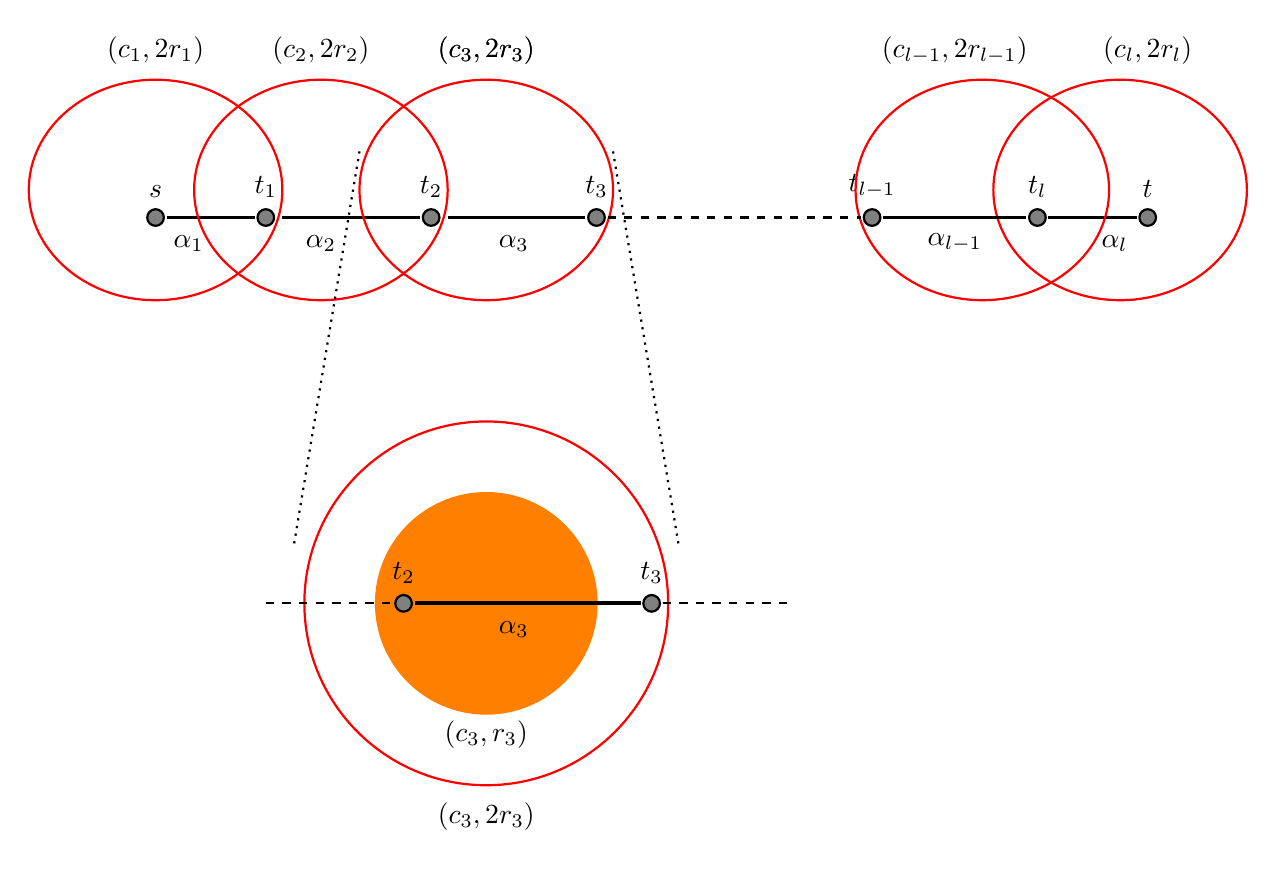
\begin{tikzpicture}[thick,scale=0.7]
	\draw (0, 0) node[circle, draw, fill=black!50, inner sep=0pt, minimum width=6pt, label = $s$] {};
	\draw (18, 0) node[circle, draw, fill=black!50, inner sep=0pt, minimum width=6pt,label = $t$] {};
	
	\draw (2, 0) node[circle, draw, fill=black!50, inner sep=0pt, minimum width=6pt,label = $t_1$] {};
	\draw [line width = 0.5mm] (0.2, 0) -- (1.8, 0);
	\draw (0.6, -1) node[red, label={$\alpha_1$}]{};
	\draw [red] (0, 0.5) ellipse (2.3 and 2);
	\draw (0, 2.4) node[red, label={$\ball(c_1, 2r_{1})$}]{};
	
	\draw (5, 0) node[circle, draw, fill=black!50, inner sep=0pt, minimum width=6pt,label = $t_2$] {};
	\draw [line width = 0.5mm] (2.3, 0) -- (4.8, 0);
	\draw (3, -1) node[red, label={$\alpha_2$}]{};
	\draw [red] (3, 0.5) ellipse (2.3 and 2);
	\draw (3, 2.4) node[red, label={$\ball(c_2, 2r_{2})$}]{};
	
	\draw (8, 0) node[circle, draw, fill=black!50, inner sep=0pt, minimum width=6pt,label = $t_3$] {};
	\draw [line width = 0.5mm] (5.3, 0) -- (7.8, 0);
	\draw (6.5, -1) node[red, label={$\alpha_3$}]{};
	\draw [red] (6, 0.5) ellipse (2.3 and 2);
	\draw (6, 2.4) node[red, label={$\ball(c_3, 2r_{3})$}]{};
	
	\draw[dotted] (3.7, 1.2) -- (2.5, -6);
	\draw[dotted] (8.3, 1.2) -- (9.5, -6);
	\draw [fill=orange,orange] (6, -7) ellipse (2 and 2);
	\draw (6, -10) node[red, label={$\ball(c_3, r_{3})$}]{};
	\draw (4.5, -7) node[circle, draw, fill=black!50, inner sep=0pt, minimum width=6pt,label = $t_2$] {};
	\draw (9, -7) node[circle, draw, fill=black!50, inner sep=0pt, minimum width=6pt,label = $t_3$] {};
	\draw [red] (6, -7) ellipse (3.3 and 3.3);
	\draw (6, -11.5) node[red, label={$\ball(c_3, 2r_{3})$}]{};
	\draw (6, 2.4) node[red, label={$\ball(c_3, 2r_{3})$}]{};
	\draw [line width = 0.5mm] (4.7, -7) -- (8.8, -7);
	\draw (6.5, -8) node[red, label={$\alpha_3$}]{};
	\draw [dashed] (2, -7) -- (4.3, -7);
	\draw [dashed] (9.2, -7) -- (11.5, -7);
	
	
	\draw (16, 0) node[circle, draw, fill=black!50, inner sep=0pt, minimum width=6pt,label = $t_l$] {};
	\draw [line width = 0.5mm] (17.8, 0) -- (16.2, 0);
	\draw (17.4, -1) node[red, label={$\alpha_l$}]{};
	\draw [red] (17.5, 0.5) ellipse (2.3 and 2);
	\draw (18, 2.4) node[red, label={$\ball(c_l, 2r_{l})$}]{};
	
	\draw (13, 0) node[circle, draw, fill=black!50, inner sep=0pt, minimum width=6pt,label = $t_{l-1}$] {};
	\draw [line width = 0.5mm] (15.8, 0) -- (13.2, 0);
	\draw (14.5, -1) node[red, label={$\alpha_{l-1}$}]{};
	\draw [red] (15, 0.5) ellipse (2.3 and 2);
	\draw (14.5, 2.4) node[red, label={$\ball(c_{l-1}, 2r_{l-1})$}]{};
	
	\draw [dashed] (8.2, 0) -- (12.8, 0); 
\end{tikzpicture}
	\end{center}
	\caption{A partitioning of the shortest path $\pi$ from $s$ to $t$ into subpaths $\alpha_1, \alpha_2, \ldots, \alpha_l$ by balls in $\clusters$. Note that in general $G[\ball(c_i, 2r_i)]$ does not necessarily contain the entire sub-path $\alpha_i$.}\label{path-partition}
\end{figure}

We prove the following simple properties of the subroutine.

\begin{observation}\label{different-balls}
	All balls in $\set{\ball(c_i, r_i)}_{1\leq i\leq l}$ are distinct.
\end{observation}
\begin{proof}
	Suppose otherwise that a ball is selected twice by \pathpart, namely $(c_i, r_i) = (c_j, r_j)$ for some $1\leq i<j\leq l$. Then, by the algorithm description we have $t_j\in \ball(c_j, 2r_j) = \ball(c_i, 2r_i)$, which contradicts the choice of $t_i$ which is the closest-to-$t$ vertex in $\ball(c_i, 2r_i)$ on $\pi$.
\end{proof}

\begin{observation}
For each $1\le i\le l$, the subpath $\alpha_i$ is entirely contained in the ball $\ball(c_i,4r_i)$.
\end{observation}
\begin{proof}
From the description of the subroutine, for each $1\le i\le l$, $s_i\in \ball(c_i, r_i)$ and $t_i\in \ball(c_i, 2r_i)$. Therefore, for every vertex $u\in \pi[s_i, t_i]$, by triangle inequality: $$\dist_{G}(c_i, u)\leq \dist_{G}(c_i, s_i) + \dist_{G}(s_i, t_i)\leq \dist_{G}(c_i, s_i) + \dist_G(c_i, s_i) + \dist_{G}(c_i, t_i)\leq 4r_i,$$
which implies that $u\in \ball(c_i, 4r_i)$.
\end{proof}

\begin{observation}\label{obs}
%Consider the moment when we have decomposed a shortest path $\pi$ as a concatenation of $\alpha_1, \alpha_2, \cdots, \alpha_l$, then we always have 
Let $R$ be the minimum radius of the balls in $\balls$. Then $l \leq |\pi|/R+1$. 
	%Plus, each path $\alpha_i$ lies within the induced subgraph $G[\ball(c_i, 4r_i)],\forall 1\leq i\leq l$.
\end{observation}
\begin{proof}
It suffices to show that, for each $1\leq i<l$, $|\alpha_i|\ge R$.
%By the algorithm description, each sub-path $\alpha_i$ is equal to $\pi[v, w]$ at some point during the iterative procedure. At the moment, the algorithm picked a ball $\ball(c, r)\in \clusters$ containing $v$, and then $w\in \pi(v, t]\cap \ball(c, 2r)$ is the closest vertex to $t$ on $\pi$ that lies in $\ball(c, 2r)$. 
From the algorithm, vertex $s_i$ belongs to the ball $\ball(c_i,r_i)$, and vertex $v_i$ is the last vertex on $\pi$ that lies in the ball $\ball(c_i,2 r_i)$, so if $t_i\neq t$ then $\dist_{G}(t_i,c_i)=2r_i$ must hold. Therefore, 
%As $i<l$, we have $w\neq t$. Then, as $w\in\ball(c, 2r)$ is the closest vertex on $\pi$ to $t$, it must be $w\in\ball^=(c, 2r)$. Then, by triangle inequality, we have:
$|\pi[s_i, t_i]|\geq \dist_{G}(c_i, t_i) - \dist_G(c_i, s_i)\geq 2r_i - r_i = r_i \geq R$.
\end{proof}


 
\paragraph{Level of balls.} Before we describe the algorithm for constructing the sets $\set{\pset_c}$, we first classify all clusters according to their sizes as follows.
Recall that we are initially given a set $\pset\subseteq V\times V$ of pairs in $G$.
For each integer $1\leq i\leq \ceil{1/\epsilon}$, we say that a ball $\ball(c, r)$ is \emph{at level $i$} iff $$n^{1-i\epsilon}/\sqrt{|\pset|}< |\ball(c, r)|\le n^{1-(i-1)\epsilon}/\sqrt{|\pset|}.$$
Denote by $\clusters_i$ the set of all level-$i$ balls in $\clusters$.
%define $$\clusters_i = \{\ball(c, r)\mid |\ball(c, r)|\in [n^{1-(i+1)\epsilon} / |P|^{1/2}, n^{1-i\epsilon}/|P|^{1/2}] \}\subseteq \clusters$$
We define the set of level-$0$ balls as $\clusters_0 = \{\ball(c, r)\mid |\ball(c, r)|> n/\sqrt{|\pset|}\}$, so $\balls=\clusters_0 \cup \clusters_1\cup\cdots\cup\clusters_{\ceil{1/\eps}}$. A ball from $\clusters$ is called \textbf{large} if it is in $\clusters_0$, and \textbf{small} otherwise. Here is a simple observation.
%Also, define parameters $K_i = \ceil{n^{(i+1)\epsilon}}$.

\iffalse
\paragraph{Phase 1: processing $\clusters_0$.} Take a random subset of vertices $S\subseteq V$ of size $\ceil{10|P|^{1/2}\log n}$. Since each ball $\ball(c, r)\in \clusters_0$ has size at least $n/|P|^{1/2}$, then with high probability, $S\cap \ball(c, r)\neq\emptyset$ for each $\ball(c, r)\in \clusters_0$. Define a path set: $$\Pi = \{\pi_{s, t}\mid s, t\in S, \dist_{G}(s, t) < 2D + 4\cdot 2^{10/\epsilon}D^{1-1/k}\}$$
For each $\ball(c, r)\in\clusters$, initialize a vertex set $U_c\leftarrow\emptyset$. 
\fi

\begin{observation}
For each $0\leq i\leq \ceil{1/\eps}$, $|\clusters_i|\leq O(n^{(i+1)\epsilon}\sqrt{|\pset|}/\epsilon)$.
\end{observation}
\begin{proof}
	By Lemma \ref{clustering}, $\sum_{\ball(c, r)\in\clusters_i}|\ball(c, r)|\leq \sum_{\ball(c, r)\in\clusters_i}|\ball(c, 4r)|\le O(n^{1+\eps}/\eps)$, and since each ball in $\bset_i$ has size at least $n^{1-i\epsilon} / \sqrt{|\pset|}$, $|\clusters_i|\leq O(n^{(i+1)\epsilon}\sqrt{|\pset|}/\epsilon)$.
\end{proof}


%\znote{some explanation}


\subsection{Step 1. Handling large balls}

We first take a uniformly random subset $S\subseteq V$ of size $\ceil{10\sqrt{|\pset|}\log n}$. Since each ball in $\clusters_0$ contains at least $n/\sqrt{|\pset|}$ vertices, with high probability, $S$ intersects all balls in $\balls_0$. 

We now proceed to iteratively construct the sets $\set{\pset_c}$ of pairs. Throughout, we maintain, for each  ball $\ball(c,r)\in \bset$, a set $\pset_c$ of pairs of vertices in $\ball(c,2r)$, and another set $U_c\subseteq S$ of vertices in $V$, which are initially empty sets. Intuitively, $U_c$ collects all vertices in $S$ whose distances from the ball center $c$ are already preserved by the spanner $H_D$ during the algorithm.

For every pair $s,t$ of vertices in $S$, we denote by $\pi_{s,t}$ an arbitrary shortest path connecting them in $G$, and we compute the set 
$$\Pi= \{\pi_{s, t}\mid s, t\in S, \text{ } \dist_{G}(s, t) < 2D + 4\cdot 2^{10/\epsilon}\cdot D^{1-1/k}\}.$$
%For each $\ball(c, r)\in\clusters$, initialize a vertex set $U_c\leftarrow\emptyset$. 

We then process all paths in $\Pi$ sequentially in an arbitrary order. For each path $\pi_{s, t}\in \Pi$, we first apply the subroutine \pathpart to it and the collection $\bset$ of balls, and obtain a partition $\pi_{s,t} = \alpha_1\circ\alpha_2\circ\cdots \circ\alpha_l$. 
For each $1\le i\le l$, we denote by $\ball(c_i, r_i)$ the ball that hosts the subpath $\alpha_i$.
If there exists a ball $\ball(c_i, r_i)$ such that $s, t\in U_{c_i}$, then we do nothing and move on to the next path in $\Pi$. Otherwise, for each $1\le  i\le l$, we add both vertices $s,t$ to the set $U_{c_i}$, and add the pair $(s_i, t_i)$ to the set $\pset_{c_i}$ of pairs.

\paragraph{Stretch analysis of Step 1.}
We make use of the following simple observation.
\begin{observation}\label{large-ball-size}
	At the end of Step 1, for each ball $\ball(c, r)\in \clusters$,  $|\pset_c|\leq |S| = \ceil{10|\pset|^{1/2}\log n}$.
\end{observation}
\begin{proof}
	By the algorithm description along with \Cref{different-balls}, every time a new pair is added to $\pset_c$, a new vertex from $S$ is also added to $U_c$. Since no more pair will be added to $\pset_{c}$ as long as $U_c$ contains all vertices of $S$, we get that $|\pset_c|\leq |U_c|\leq |S| = \ceil{10|\pset|^{1/2}\log n}$.
\end{proof}

%As the beginning of our stretch analysis, 
We now show in the following claims that, after the first step, all pairwise distances (in $G$) between vertices in $S$ are well-preserved in $H_D$. And as the set $S$ hits all balls in $\bset_0$ with high probability, the distance between any pair of vertices from $V(\balls_0)$ is also well-preserved.
% As $S$ hits every ball in $\bset_0$, this implies that the distance (in $G$) between every pair of vertices in $V(\bset_0)$ is well-preserved.

\begin{claim}\label{C0}
%During the enumeration of paths from $\Pi$, for any vertex $s\in S$ and ball $\ball(c, r)\in \clusters$, 
After a vertex $s\in S$ is added to the set $U_c$ for some $\ball(c,r)\in \bset$, the following holds:
	$$\dist_{H_D}(s, c)\leq \dist_G(s, c) + 49\cdot 2^{(30k-10)/\epsilon}\cdot D^{1-1/k}.$$
\end{claim}
\begin{proof}
Assume that the shortest path $\pi_{s,t}$ was being processed when $s$ was added to $U_c$, and that $\ball(c, r)$ was $\ball(c_i, r_i)$ under the notation of the subroutine \pathpart. From the algorithm, for each $1\leq j\leq l$, the pair $(s_j, t_j)$ was added to the collection $\pset_{c_j}$. From the construction of $H_D$, for each $1\leq j\leq l$, there exists a path $\phi_j$ in $H_D$ from $s_j$ to $t_j$, such that: 
	$$\begin{aligned}
	|\phi_j| \leq |\alpha_j| + 2^{30(k-1)/\epsilon}\cdot |\alpha_j|^{1-1/(k-1)} &\leq |\alpha_j| + 2^{30(k-1)/\epsilon}\cdot \left(4\cdot 2^{10/\epsilon}\cdot D^{1-1/k}\right)^{1-1/(k-1)}\\
	&\leq |\alpha_j| + 4\cdot 2^{(30k-20)/\epsilon}\cdot D^{1-2/k}
	\end{aligned}$$
	(we have used the fact that $|\alpha_j| < \dist_G(s_j,t_j)\le \dist_G(s_j,c_j)+ \dist_G(t_j,c_j)\le  4r_{j} \leq 4\cdot 2^{10/\epsilon}\cdot D^{1-1/k}$). Taking a summation over all indices $1\leq j\leq i$ and using  \Cref{obs}, we have:
	$$\begin{aligned}
	\dist_{H_D}(s, c_i)&\leq  \dist_{H_D}(c_i, t_i)+ \dist_{H_D}(s, t_i)\\
	&\leq 2\cdot 2^{10/\epsilon}\cdot D^{1-1/k} + \dist_G(s, t_i) + 48\cdot 2^{(30k-10)/\epsilon}\cdot D^{1-1/k}\\
	&\leq 2\cdot 2^{10/\epsilon}\cdot D^{1-1/k} + (\dist_G(s, c_i) + \dist_G(c_i, t_i)) + 48\cdot 2^{(30k-10)/\epsilon}\cdot D^{1-1/k}\\
	&\leq \dist_G(s, c_i) + 49\cdot 2^{(30k-10)/\epsilon} \cdot D^{1-1/k}.
	\end{aligned}$$
\end{proof}

\begin{claim}\label{C0-ineq}
	For any $s, t\in S$ such that $\dist_G(s, t) < 2D + 4\cdot 2^{10/\epsilon}\cdot D^{1-1/k}$, we have:
	$$\dist_{H_D}(s, t)\leq \dist_G(s, t) + 100 \cdot 2^{(30k-10)/\epsilon}\cdot D^{1-1/k}.$$
\end{claim}
\begin{proof}
For any such pair of vertices $s, t\in S$, consider the moment when the shortest path $\pi_{s, t}\in \Pi$ was processed and partitioned into subpaths $\alpha_1,\ldots,\alpha_l$. We distinguish between the following two cases.
	\begin{itemize}[leftmargin=*]
		\item Case 1. There existed an index $1\le i\le l$ such that $s, t\in U_{c_i}$ at the moment.
		
		In this case, from \Cref{C0}:
		$$\dist_{H_D}(s, c_i)\leq \dist_G(s, c_i) + 49\cdot 2^{(30k-10)/\epsilon} \cdot D^{1-1/k}\leq \dist_G(s, s_i) + 50\cdot 2^{(30k-10)/\epsilon} \cdot D^{1-1/k},$$
		$$\dist_{H_D}(c_i, t)\leq \dist_G(c_i, t) +49\cdot 2^{(30k-10)/\epsilon}\cdot D^{1-1/k}\leq \dist_G(s_i, t) + 50\cdot 2^{(30k-10)/\epsilon}\cdot D^{1-1/k}.$$
		Summing up these two inequalities finishes the proof.
		
		\item Case 2. There did not exist any $i$ such that $s, t\in U_{c_i}$ at the moment.
		
		In this case, for each $1\leq j\leq l$, the pair $(s_j, t_j)$ was added to the set $\pset_{c_j}$. Similar to the proof of \Cref{C0}, for each $1\leq j\leq l$, there exists a path $\phi_j$ in $H_D$ from $s_j$ to $t_j$, such that: 
		$$\begin{aligned}
		|\phi_j| \leq |\alpha_j| + 2^{30(k-1)/\epsilon}\cdot |\alpha_j|^{1-1/(k-1)} &\leq |\alpha_j| + 2^{30(k-1)/\epsilon}\cdot \left(4\cdot 2^{10/\epsilon}\cdot D^{1-1/k}\right)^{1-1/(k-1)}\\
		&\leq |\alpha_j| + 4\cdot 2^{(30k-20)/\epsilon}\cdot D^{1-2/k}.
		\end{aligned}$$
		Taking a summation for all indices $1\leq j\leq l$ and using \Cref{obs}, we get that:
		$$\dist_{H_D}(s, t) \leq \dist_G(s, t) + 48\cdot 2^{(30k-10)/\epsilon} \cdot D^{1-1/k}.$$
	\end{itemize}
\end{proof}




\subsection{Step 2. Handling small balls} 

We now process all pairs $(s,t)\in \pset$ with $D\le \dist_G(s, t) < 2D$ in an arbitrary order. Take any such pair $(s,t)$, and compute a shortest path $\pi_{s,t}$ between them in $G$. We then apply the subroutine \pathpart to it and the collection $\bset$ of balls, and obtain a partitioning $\pi_{s,t} = \alpha_1\circ\alpha_2\circ\cdots \circ\alpha_l$ together with the balls $\set{\ball(c_i, r_i)}_{1\le i\le l}$ that host them. However, as the number of pairs $(s,t)\in \pset$ with $D\le \dist_G(s, t) < 2D$ can be very large, we cannot afford to add the pair $(s_i,t_i)$ to set $\pset_{c_i}$ for all $1\le i\le l$ as in Step 1, and will instead carefully pick a subset of indices in $[1,l]$ to do so.


%Go over each demand pair $(s, t)\in P$ such that $\dist_G(s, t)\in [D, 2D)$ in an arbitrary order. In each round, a pair $(s, t)\in P$ is enumerated, and let $\pi$ be a shortest path between $s, t$. Apply the path partition subroutine to obtain sub-paths $\alpha_1, \alpha_2, \cdots, \alpha_l$ and balls $\ball(c_1, r_{c_1}), \ball(c_2, r_{c_2}), \cdots, \ball(c_l, r_{c_l})$. 



%For the rest of this round, we will be adding some pairs $(s_i, t_i)$ to $P_{c_i}$. During the process, each index $i\in [1, l]$ has two fields:
\iffalse
\begin{itemize}
	\item \textbf{Marked} or \textbf{unmarked}
	
	Index $i$ is marked if $(s_i, t_i)$ has already been added to $P_{c_i}$; otherwise $i$ is unmarked.
	
	\item \textbf{Ranks}
	
	Then level of index $i$ is equal to $\rk$ if $\ball(r_i, c_{r_i})\in\clusters_\rk$.
\end{itemize}
\fi

We will now describe how to choose these indices. This is again done via an iterative process. Throughout, we will gradually construct a binary tree $\tree$, which initially contains a single node, which is the root of $\tree$. 
Each node of the tree is labeled by a subinterval of $[1, l]$. Initially, the root of $\tree$ is labeled with $[1, l]$. %The tree $\tree$ is grown downward by a repetitive procedure.
Each index $i\in [1,l]$ is either marked \textbf{active} or \textbf{inactive}. Initially, all indices are inactive. The algorithm continues to be executed unless for each leaf of the tree $\tree$, all indices in its associated interval are active. Over the course of the algorithm, whenever we mark some index $i$ active, we will simultaneously add the pair $(s_i,t_i)$ to the set $\pset_{c_{i}}$.
We say that an index $i\in [1,l]$ is \textbf{at level $j$} iff its corresponding ball $\ball(c_i,r_i)$ is at level $j$ (that is, if $n^{1-j\epsilon}/\sqrt{|\pset|}< |\ball(c_i, r_i)|\le n^{1-(j-1)\epsilon}/\sqrt{|\pset|}$).

As a pre-processing step, we first focus on level-$0$ indices (if there are none of them, then we skip the pre-processing). Let $i_1, i_2$ be the smallest and the largest level-$0$ indices, respectively. We add two new nodes to the tree $\tree$, connecting each of them to the root by an edge. One of the new nodes is labeled by interval $[1, i_1-1]$, and the other node is labeled by interval $[i_2+1, l]$. So now the levels of indices on $[1, i_1-1]$ and $[i_2+1, l]$ are at least $1$. Here we do not modify the active/inactive status of the indices.

%The repetitive procedure is as follows. At the root of $\tree$ we first perform one step of preprocessing. If there is a sub-path $\alpha_i$ with level $0$, then let $i_1, i_2$ be the smallest and the largest indices such that $i_1, i_2$ have level $0$. Then, grow two children $N_1, N_2$ associated with interval $[1, i_1]$ and $[i_2, l]$, respectively. 

%For the rest, each time pick an arbitrary node $N$ which is currently is a leaf containing some unmarked indices; if such node $N$ does not exist anymore, the construction of $\tree$ is complete. Denote by $[i', i'']$ the interval associated with $N$.

%We the process level-$i$ indices sequentially for $i=1,\ldots,\ceil{1/\eps}$.

We now describe an iteration. We take an arbitrary leaf of the tree $\tree$ that whose associated interval contains an inactive index, and denote by $I$ the interval associated with this leaf node. We can assume that all levels of $I$ are at least $1$.
For each $1\le L\le \ceil{1/\eps}$, let $i^L_1 < i^L_2 <\cdots < i^L_{p(L)}$ be all level-$L$ indices in the interval $I$ (so the number of level-$L$ indices in $I$ is $p(L)$); we will \textbf{ignore the superscript $L$} if it is clear from context. Consider the corresponding balls $\set{\ball(c_{i^L_a}, r_{i^L_a})}$ that host them. We say that a pair $\left(\ball(c_{i^L_a}, r_{i^L_a}), \ball(c_{i^L_b}, r_{i^L_b})\right)$ of balls is \textbf{tight}, iff 
$$\dist_{H_D}(c_{i^L_a}, c_{i^L_b}) \le \dist_G(c_{i^L_a}, c_{i^L_b}) + \left(3\cdot 2^{(30k-20)/\epsilon} + 10\cdot 2^{10/\epsilon}\right)\cdot D^{1-1/k}.$$
and we denote by $q(L)$ the number of pairs of balls in $\set{\ball(c_{i^L_a}, r_{i^L_a})}$ which are not tight. In addition, we define $\beta(L)=\ceil{n^{(L+1)\epsilon}}$.

We will distinguish between the following two cases.

\begin{comment}
	\iffalse
	We will classify all unmarked levels into two different types. For any level-$L$ such that interval $[i', i'']$ contains some unmarked indices of level $L$, let $x\leq i_1 < i_2 <\cdots < i_p\leq y$ be all such indices.  Let $q$ be the total number of pairs of balls $(\ball(c_{i_a}, r_{c_{i_a}}), \ball(c_{i_b}, r_{c_{i_b}})), 1\leq a<b\leq p$ such that:
	$$\dist_{H_D}(c_{i_a}, c_{i_b}) > \dist_G(c_{i_a}, c_{i_b}) + \left(3\cdot 2^{(30k-20)/\epsilon} + 10\cdot 2^{10/\epsilon}\right)D^{1-1/k}$$
	To classify this level $\rk$ as Type (A) or Type (B), it depends on the comparison between $p$ and $q$.
	\begin{enumerate}[(A)]
		\item $p \leq \max\{4\cdot \ceil{n^{(\rk+1)\epsilon}}, 8q /\ceil{n^{(\rk+1)\epsilon}} \}$.
		
		\item $p > \max\{4\cdot \ceil{n^{(\rk+1)\epsilon}}, 8q /\ceil{n^{(\rk+1)\epsilon}} \}$.
	\end{enumerate}
	
	The algorithm takes the following branching depending on types of levels within $[i', i'']$.
	\fi
\end{comment}

\paragraph{Case 1. For all $1\le L\le \ceil{1/\eps}$, $p(L) \leq \max\{4\beta(L), 8q(L)/\beta(L) \}$.}
In this case, we activate all indices $i\in I$ (and along with it add the corresponding pair $(s_{i}, t_{i})$ to the set $\pset_{c_{i}}$ and then update $H_D$ accordingly), and continue to the next iteration. We do not modify the tree $\tree$ in this iteration. Note that, after this iteration, the associated interval of the leaf that we processed in this iteration no longer contains any inactive indices, so it will remain a leaf in $\tree$ forever.

\paragraph{Case 2. There exists some $1\le L\le \ceil{1/\eps}$, such that $p(L) > \max\{4\beta(L), 8q(L)/\beta(L) \}$.}
In this case, 
%for each $a\in [1, \beta(L)]\cup [p(L)-\beta(L)+1, p(L)]$, 
we activate the $\beta(L)$ smallest and $\beta(L)$ largest level-$L$ indices in $I$ (and along with it add the corresponding pair $(s_{i}, t_{i})$ to the set $\pset_{c_{i}}$ and then update $H_D$ accordingly).

In order to describe the modification of $\tree$ in this iteration, we need the following lemma.

%To proceed with the rest of this iteration of growing $\tree$, we need to first state an important property.
\begin{lemma}
	There exists three level-$L$ indices $i_x, i_y, i_z\in I$ such that:
	\begin{enumerate}[(i)]
		\item $1\leq x\leq \beta(L)$;
		\item $p(L)-\beta(L) < y\leq p(L)$;
		\item $\beta(L) < z\leq p(L)-\beta(L)$;
		\item the pair $\left(\ball(c_{i_x}, r_{i_x}),\ball(c_{i_z}, r_{i_z})\right)$ and the pair $\left(\ball(c_{i_y}, r_{i_y}),\ball(c_{i_z}, r_{i_z})\right)$ of balls are both tight.
	\end{enumerate}
\end{lemma}
\begin{proof}
	Assume for contradiction that there do not exist such three indices. Consider now any pair $a,b$ of indices such that $1\le a\le \beta(L)$ and $\beta(L) < b \leq p(L) - \beta(L)$. From our assumption, for at least one pair of indices $(i^L_a,i^L_{b})$ and $(i^L_b,i^L_{p(L)+1-a})$, their corresponding balls are not tight.
	This implies that $q(L)\geq (p(L) - 2\beta(L))\cdot\beta(L)$. Then either $p(L)<4\beta(L)$ holds, or $q(L)\geq p(L)\cdot \beta(L) / 8$ holds, a contradiction of the initial assumption of Case 2.
	\iffalse
	Suppose the statement does not hold. Then, for any triple of indices: 
		$$x\in [1, K_\rk], y = p+1 - x\in [p-K_\rk+1, p], z\in [K_\rk+1, p-K_\rk]$$
		We know that at least one of the following two inequalities hold:
		$$\dist_{H_D}(c_{i_{x}}, c_{i_{z}})> \dist_G(c_{i_{x}}, c_{i_{z}}) + \left(3\cdot 2^{(30k-20)/\epsilon} + 10\cdot 2^{10/\epsilon}\right)D^{1-1/k}$$
		$$\dist_{H_D}(c_{i_{z}}, c_{i_{y}})> \dist_G(c_{i_{z}}, c_{i_{y}}) + \left(3\cdot 2^{(30k-20)/\epsilon} + 10\cdot 2^{10/\epsilon}\right) D^{1-1/k}$$
		
		Hence, for any $x\in [1, K_\rk], z\in [K_\rk+1, p-K_\rk]$, either the pair $(\ball(c_{i_{x}}, r_{c_{i_{x}}}), \ball(c_{i_{z}}, r_{c_{i_{z}}}))$ should contribute to the counting of $q$, or $(\ball(c_{i_{y}}, r_{c_{i_{y}}}), \ball(c_{i_{z}}, r_{c_{i_{z}}}))$ should do so. Therefore, $q\geq (p - 2K_\rk)\cdot K_\rk \geq p\cdot K_\rk / 8$, which is a contradiction of the definition of Type (B).
	\fi
\end{proof}

To complete this iteration, we pick indices $i_x, i_y, i_z$ as in the above lemma. We then add two new nodes to the tree $\tree$ (together with an edge connecting to the leaf) as the child nodes of this leaf. 
Denote $I=[i',i'']$, and we label the child nodes with intervals $[i', i_{x}]$ and $[i_{y}, i'']$, respectively. This completes the description of an iteration. See Figure \ref{bridge} for an illustration.


\begin{figure}[h]
	\begin{center}
		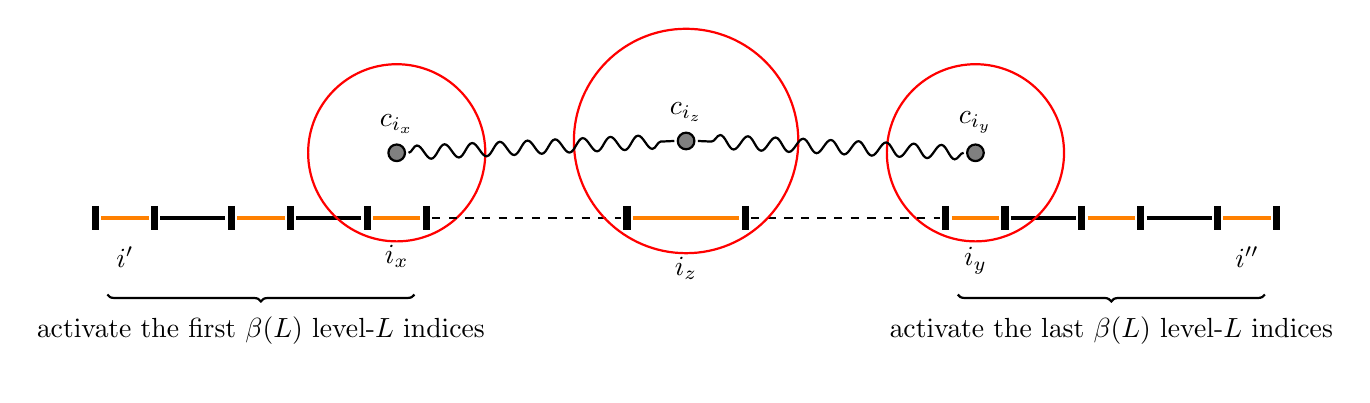
\begin{tikzpicture}[thick,scale=0.75]
	\draw [line width = .9mm] (0, 0.2) -- (0, -0.2);
	\draw [line width = .9mm] (1, 0.2) -- (1, -0.2);
	\draw [line width = 0.5mm, color=orange] (0.1, 0) -- (0.9, 0);
	\draw (0.5, -1.2) node[red, label={$i'$}]{};
	
	\draw [line width = 0.5mm] (1.1, 0) -- (2.2, 0);
	
	\draw [line width = .9mm] (2.3, 0.2) -- (2.3, -0.2);
	\draw [line width = .9mm] (3.3, 0.2) -- (3.3, -0.2);
	\draw [line width = 0.5mm, color=orange] (2.4, 0) -- (3.2, 0);
	%\draw (2.8, -1.2) node[red, label={$x+1$}]{};
	
	\draw [line width = 0.5mm] (3.4, 0) -- (4.5, 0);
	
	\draw [line width = .9mm] (4.6, 0.2) -- (4.6, -0.2);
	\draw [line width = .9mm] (5.6, 0.2) -- (5.6, -0.2);
	\draw [line width = 0.5mm, color=orange] (4.7, 0) -- (5.5, 0);
	\draw (5.1, -1.2) node[red, label={$i_{x}$}]{};
	\draw [red] (5.1, 1.1) ellipse (1.5 and 1.5);
	\draw (5.1, 1.1) node[circle, draw, fill=black!50, inner sep=0pt, minimum width=6pt, label = $c_{i_{x}}$] {};
	
	\draw [decorate,
	decoration = {brace}] (5.4,-1.3) -- (0.2,-1.3);
	\draw (2.8, -2.5) node[label={activate the first $\beta(L)$ level-$L$ indices}]{};
	
	\draw [line width = .9mm] (20, 0.2) -- (20, -0.2);
	\draw [line width = .9mm] (19, 0.2) -- (19, -0.2);
	\draw [line width = 0.5mm, color=orange] (19.1, 0) -- (19.9, 0);
	\draw (19.5, -1.2) node[red, label={$i''$}]{};
	
	\draw [line width = 0.5mm] (17.8, 0) -- (18.9, 0);
	
	\draw [line width = .9mm] (17.7, 0.2) -- (17.7, -0.2);
	\draw [line width = .9mm] (16.7, 0.2) -- (16.7, -0.2);
	\draw [line width = 0.5mm, color=orange] (16.8, 0) -- (17.6, 0);
	%\draw (17.2, -1.2) node[red, label={$y-1$}]{};
	
	\draw [line width = 0.5mm] (15.5, 0) -- (16.6, 0);
	
	\draw [line width = .9mm] (15.4, 0.2) -- (15.4, -0.2);
	\draw [line width = .9mm] (14.4, 0.2) -- (14.4, -0.2);
	\draw [line width = 0.5mm, color=orange] (14.5, 0) -- (15.3, 0);
	\draw (14.9, -1.3) node[red, label={$i_{y}$}]{};
	\draw [red] (14.9, 1.1) ellipse (1.5 and 1.5);
	\draw (14.9, 1.1) node[circle, draw, fill=black!50, inner sep=0pt, minimum width=6pt, label = $c_{i_{y}}$] {};
	
	\draw [decorate,
	decoration = {brace}] (19.8,-1.3) -- (14.6,-1.3);
	\draw (17.2, -2.5) node[label={activate the last $\beta(L)$ level-$L$ indices}]{};
	
	\draw [dashed] (5.7, 0) -- (8.9, 0);
	\draw [line width = .9mm] (9, 0.2) -- (9, -0.2);
	\draw [line width = .9mm] (11, 0.2) -- (11, -0.2);
	\draw [line width = 0.5mm, color=orange] (9.1, 0) -- (10.9, 0);
	\draw (10, -1.4) node[red, label={$i_{z}$}]{};
	\draw [dashed] (11.1, 0) -- (14.3, 0);

	\draw [red] (10, 1.3) ellipse (1.9 and 1.9);
	\draw (10, 1.3) node[circle, draw, fill=black!50, inner sep=0pt, minimum width=6pt, label = $c_{i_{z}}$] {};
	
	\draw [style={decorate, decoration=snake}] (5.3, 1.1) -- (9.8, 1.3);
	\draw [style={decorate, decoration=snake}] (14.7, 1.1) -- (10.2, 1.3);
\end{tikzpicture}
	\end{center}
	\caption{The distances between $c_{i_{x}}, c_{i_{z}}$ and $c_{i_{y}}, c_{i_{z}}$ are approximately preserved in $H$; the orange segments correspond to level-$L$ indices; a prefix and a suffix of level-$L$ indices are activated in this iteration.}\label{bridge}
\end{figure}

%\subsection{Stretch analysis}

\iffalse
The following simple observation is the key to our analysis.
\begin{lemma}\label{obs0}
	Consider the moment when we have decomposed a shortest path $\pi$ as a concatenation of $\alpha_1, \alpha_2, \cdots, \alpha_l$, then we always have $l \leq \ceil{\frac{|\pi|}{D^{1-1/k}}}$. 
	%Plus, each path $\alpha_i$ lies within the induced subgraph $G[\ball(c_i, 4r_i)],\forall 1\leq i\leq l$.
\end{lemma}
\begin{proof}
	It suffices to show that each sub-path $\alpha_i, \forall 1\leq i<l$ has length at least $D^{1 - 1/k}$. By the algorithm description, each sub-path $\alpha_i$ is equal to $\pi[v, w]$ at some point during the iterative procedure. At the moment, the algorithm picked a ball $\ball(c, r)\in \clusters$ containing $v$, and then $w\in \pi(v, t]\cap \ball(c, 2r)$ is the closest vertex to $t$ on $\pi$ that lies in $\ball(c, 2r)$. 
	
	As $i<l$, we have $w\neq t$. Then, as $w\in\ball(c, 2r)$ is the closest vertex on $\pi$ to $t$, it must be $w\in\ball^=(c, 2r)$. Then, by triangle inequality, we have:
	$$|\pi[v, w]|\geq \dist_{G}(c, w) - \dist_G(c, v)\geq 2r - r = r \geq D^{1-1/k}$$
\end{proof}
\fi


\paragraph{Stretch analysis of Step 2.}
Consider any pair $(s, t)\in \pset$ such that $D\le \dist_G(s, t) < 2D$. Let $\pi$ be the shortest path connecting $s$ to $t$ that was processed in Step 2. We start by showing that, in this iteration, the depth of the tree $\tree$ that we construct is small. 

\begin{observation}
At the end of the iteration of processing $\pi$, $\tree$ has depth at most $\ceil{1/\eps}+1$.
\end{observation}
\begin{proof}
The pre-processing step can increase the depth by at most one. From the algorithm description, it is easy to observe that, as we walk down in any root-to-leaf path in $\tree$, in each step, the number of levels with inactive indices decreases by one. Hence, the observation follows.
%For the rest we only consider general steps that take the branching (1)(2). Consider any iteration where the algorithm picked a node $N$ which was a leaf containing some unmarked indices back then. If the algorithm took branch (1), then all indices from $[i', i'']$ would be marked immediately, and node $N$ would stay a leaf for the rest. If the algorithm took branch (2), then by the algorithm description, all indices with level $\rk$ within intervals $[i', i_{x}]$ and $[i_{y}, i'']$ are marked, hence the number of levels of unmarked indices in children $N_1, N_2$ decreases by at least one. Since the total number of levels is $\ceil{1/\eps}$, the maximum depth of $\tree$ in the end is at most $\ceil{1/\eps} + 1$.
\end{proof}

We are now ready to analyze the stretch (in $H_D$) of pairs in $\pset$.

\begin{lemma}
\label{lem: step 2}
For every pair $(s, t)\in \pset$, $\dist_{H_D}(s, t)\leq \dist_G(s, t) + 2^{30k/\epsilon}\cdot D^{1-1/k}$.
\end{lemma}
\begin{proof}
	We will utilize the tree structure of $\tree$. Focus on the time when the construction of $\tree$ was completed. For any tree node $N$, its \emph{height} is defined to be the maximum depth of the subtree of $\tree$ rooted at $N$. We first prove the following claim.
	
	\begin{claim}
	\label{clm: stretch by depth}
		For each non-root tree node $N$ with height $h$ and associated interval $[i', i'']$,
		$$\dist_{H_D}(c_{i'}, c_{i''})\leq \dist_G(c_{i'}, c_{i''}) + 30\cdot (2^{h+1}-1)\cdot 2^{(30k-20)/\epsilon}\cdot D^{1-1/k}.$$
	\end{claim}
	\begin{proof}[Proof of \Cref{clm: stretch by depth}]		
%	\znote{$i,i''$.}	
	We prove the claim by induction on $h$. The base case is when $h = 0$ and $N$ is a leaf in $\tree$. From the algorithm, for each $i\in [i', i'']$, the pair $(s_i, t_i)$ is added into the set $\pset_{c_i}$. Similar to the proof of \Cref{C0}, for each $i'\leq i\leq i''$, there exists a path $\phi_i$ in $H_D$, such that 
		$$\begin{aligned}
			|\phi_j| \leq |\alpha_j| + 2^{30(k-1)/\epsilon}\cdot |\alpha_j|^{1-1/(k-1)} &\leq |\alpha_j| + 2^{30(k-1)/\epsilon}\cdot \left(4\cdot 2^{10/\epsilon}\cdot D^{1-1/k}\right)^{1-1/(k-1)}\\
			&\leq |\alpha_j| + 4\cdot 2^{(30k-20)/\epsilon}\cdot D^{1-2/k}.
		\end{aligned}$$
		Taking a summation and using \Cref{obs} (which implies that $l<3D^{1/k}$),
		$$\dist_{H_D}(s_{i'}, t_{i''})\leq \dist_G(s_{i'}, t_{i''}) + 12\cdot 2^{(30k-20)/\epsilon}\cdot D^{1-1/k}.$$
		By triangle inequality, we have:
		$$\dist_{H_D}(s_{i'}, t_{i''})\geq \dist_{H_D}(c_{i'}, c_{i''}) - \dist_{H_D}(c_{i'}, s_{i'}) - \dist_{H_D}(c_{i''}, t_{i''})\geq \dist_{H_D}(c_{i'}, c_{i''}) - 3\cdot 2^{10/\epsilon}D^{1-1/k},$$
		$$\dist_G(s_{i'}, t_{i''})\leq \dist_G(c_{i'}, c_{i''}) + \dist_G(c_{i'}, s_{i'}) + \dist_G(c_{i''}, t_{i''})\leq \dist_G(c_{i'}, c_{i''}) + 3\cdot 2^{10/\epsilon}D^{1-1/k}.$$
		Combining all three inequalities, we have:
		$$\begin{aligned}
			\dist_{H_D}(c_{i'}, c_{i''})&\leq \dist_G(c_{i'}, c_{i''}) + \left(12\cdot 2^{(30k-20)/\epsilon} + 6\cdot 2^{10/\epsilon}\right)\cdot D^{1-1/k}\\
			&< \dist_G(c_{i'}, c_{i''}) + 30\cdot 2^{(30k-20)/\epsilon}\cdot D^{1-1/k}.
		\end{aligned}$$
		
		Assume now that the claim is true for $1,\ldots,h-1$. Consider a node $N$ at height $h$ with two children $N_1, N_2$ associated with intervals $[i', i_{x}]$ and $[i_{y}, i'']$ respectively. By inductive hypothesis, we have:
		$$\dist_{H}(c_{i'}, c_{i_{x}})\leq \dist_G(c_{i'}, c_{i_{x}}) + 30\cdot (2^{h}-1)\cdot 2^{(30k-20)/\epsilon}\cdot D^{1-1/k},$$
		$$\dist_{H}(c_{i''}, c_{i_{y}})\leq \dist_G(c_{i''}, c_{i_{y}}) + 30\cdot (2^{h}-1)\cdot 2^{(30k-20)/\epsilon}\cdot D^{1-1/k}.$$
		From the algorithm, the node $N$ may only grow two children $N_1$ and $N_2$ in Case 2, and in this case there exists an index $i_z$ such that the pairs $(\ball(c_{i_x}, r_{i_x}),\ball(c_{i_z}, r_{i_z}))$ and $(\ball(c_{i_y}, r_{i_y}),\ball(c_{i_z}, r_{i_z}))$ of balls are both tight. In other words,
		\[\dist_{H_D}(c_{i_{x}}, c_{i_{z}})\leq \dist_G(c_{i_{x}}, c_{i_{z}}) + \left(3\cdot 2^{(30k-20)/\epsilon} + 10\cdot 2^{10/\epsilon}\right)D^{1-1/k},\]
		\[\dist_{H_D}(c_{i_{z}}, c_{i_{y}})\leq \dist_G(c_{i_{z}}, c_{i_{y}}) + \left(3\cdot 2^{(30k-20)/\epsilon} + 10\cdot 2^{10/\epsilon}\right)D^{1-1/k}.\]
		The sum of the left-hand sides of the above four inequalities is at least $\dist_{H_D}(c_{i'}, c_{i''})$, from triangle inequality. For their right-hand sides, notice that: 
		\[\begin{aligned}
			\dist_G(c_{i'}, c_{i_{x}}) + \dist_G(c_{i_{x}}, c_{i_{z}})&\leq (\dist_G(s_{i'}, s_{i_{x}}) + \dist_G(c_{i'}, s_{i'}) + \dist_G(c_{i_{x}}, s_{i_{x}}))\\
			& +(\dist_G(s_{i_{x}}, s_{i_{z}}) + \dist_G(c_{i_{x}}, s_{i_{x}}) + \dist_G(c_{i_{z}}, s_{i_{z}}))\\
			&\leq \dist_G(s_{i'}, s_{i_{z}}) + 4\cdot 2^{10/\epsilon}\cdot D^{1-1/k}\\
			&\leq \dist_G(c_{i'}, c_{i_{z}}) + 6\cdot 2^{10/\epsilon}\cdot D^{1-1/k}.
		\end{aligned}
		\]
		Symmetrically, we also have $\dist_G(c_{i''}, c_{i_{y}}) + \dist_G(c_{i_{y}}, c_{i_{z}})\leq \dist_G(c_{i''}, c_{i_{z}}) + 6\cdot 2^{10/\epsilon}\cdot D^{1-1/k}$.
		
		Note that
		$\dist_G(c_{i'}, c_{i_{z}}) + \dist_G(c_{i''}, c_{i_{z}})\leq \dist_G(c_{i'}, c_{i''}) + 2\cdot 2^{10/\epsilon}\cdot D^{1-1/k}$ (again by triangle inequality). Altogether, we get that:
		$$\dist_{H_D}(c_{i'}, c_{i''})\leq \dist_G(c_{i'}, c_{i''}) + 30\cdot (2^{h+1}-1)\cdot 2^{(30k-20)/\epsilon}\cdot D^{1-1/k}.$$
	\end{proof}

	Lastly, we consider the root $N_0$ of $\tree$. Recall that it is associated with the interval $[1,l]$. 
	If there are no level-$0$ indices in $[1, l]$, then \Cref{clm: stretch by depth} already implies \Cref{lem: step 2}. We assume from now on that there are level-$0$ indices in $[1, l]$. From the algorithm, in the pre-processing step, $N_0$ grows two children $N_1, N_2$ associated with intervals $[1, i_1-1]$ and $[i_2+1, l]$, respectively, such that $i_1, i_2$ are the smallest and the largest level-$0$ indices. By definition of $S$, there exists $v_1, v_2$ such that $v_1\in (\ball(c_{i_1}, r_{i_1})\cap S), v_2\in (\ball(c_{i_2}, r_{i_2})\cap S)$. Notice that $\dist_G(v_1, v_2)\leq \dist_G(s_{i_1}, s_{i_2}) + 4\cdot 2^{10/\epsilon}\cdot D^{1-1/k} < 2D + 4\cdot 2^{10/\epsilon}\cdot D^{1-1/k} $. Then, from \Cref{C0-ineq}, we have:
	$$\dist_{H_D}(v_1, v_2)\leq \dist_G(v_1, v_2) + 100\cdot 2^{(30k-10)/\epsilon} D^{1-1/k}.$$
	
	Suppose $N_1, N_2$ have height $h_1, h_2\leq \ceil{1/\eps}$ respectively. By \Cref{clm: stretch by depth},
	$$\dist_{H_D}(c_1, c_{i_1-1})\leq \dist_G(c_1, c_{i_1-1}) + 30\cdot (2^{h_1+1}-1)\cdot 2^{(30k-20)/\epsilon}\cdot D^{1-1/k},$$
	$$\dist_{H_D}(c_l, c_{i_2+1})\leq \dist_G(c_l, c_{i_2+1}) + 30\cdot (2^{h_2+1}-1)\cdot 2^{(30k-20)/\epsilon}\cdot D^{1-1/k}.$$
%
Taking a summation of the left-hand sides of the above three inequalities:
	\[\begin{aligned}
		&\dist_{H_D}(c_1, c_{i_1-1}) + \dist_{H_D}(c_l, c_{i_2+1}) + \dist_{H_D}(v_1, v_2)\\
		& \geq \dist_{H_D}(c_1, c_{i_1-1}) + \dist_{H_D}(c_l, c_{i_2+1}) + \dist_{H_D}(c_{i_1}, c_{i_2}) - 2\cdot 2^{10/\epsilon}\cdot D^{1-1/k}\\
		&\geq \dist_{H_D}(c_1, c_l) - 8\cdot 2^{10/\epsilon}\cdot D^{1-1/k}\\
		&\geq \dist_{H_D}(s, t) - 11\cdot 2^{10/\epsilon} D^{1-1/k}.
	\end{aligned}\]
%
Taking a summation of their right-hand sides (ignoring the tails for now):
	\[\begin{aligned}
		\dist_G(c_1, c_{i_1-1}) + \dist_G(c_l, c_{i_2+1}) + \dist_G(v_1, v_2) & \leq \dist_G(s, s_{i_1-1}) + (\dist_G(s, c_1) + \dist_G(c_{i_1-1}, s_{i_1}))\\
		&+\dist_G(t, s_{i_2+1}) + (\dist_G(t, c_l) + \dist_G(s_{i_2+1}, c_{i_2}))\\
		&+ \dist_G(s_{i_1}, s_{i_2}) + (\dist_G(v_1, s_{i_1}) + \dist_G(v_2, s_{i_2}))\\
		&\leq \dist_G(s, t) + 9\cdot 2^{10/\epsilon}\cdot D^{1-1/k}.
\end{aligned} \]
%
Altogether, $\dist_{H_D}(s, t)\leq \dist_G(s, t) + 200\cdot 2^{(30k-10)/\epsilon}D^{1-1/k} < \dist_G(s, t) + 2^{30k/\epsilon}D^{1-1/k}$.
%Finally, if $[1, l]$ does not contain any level-$0$ indices, then we can prove the above inequality in a similar manner based on the inductive claim.
\end{proof}

\subsection{Size analysis}

In this subsection, we complete the proof of \Cref{pairwise-sublinear} by showing that the spanner $H$ constructed by the algorithm in this section satisfies the desired size bound. We start by proving the following claim.

\begin{claim}
\label{clm: pairs added}
In the end, for each level $1\leq i\leq \ceil{1/\eps}$, $\sum_{\ball(c, r)\in \clusters_i}|\pset_c|\leq O(\frac{1}{\epsilon^2}2^{\ceil{1/\epsilon}}n^{(i+1)\epsilon}|\pset|\log n)$.
\end{claim}
\begin{proof}
%For $i = 0$, note that the algorithm never increases $|\pset_c|$ when $\ball(c, r)\in \clusters_0$ during Step 2, so by \Cref{large-ball-size}, $|\pset_c|\leq O(|\pset|^{1/2}\log n)$. Since $|\clusters_0|\leq O(n^\epsilon |\pset|^{1/2}/\epsilon)$, the inequality holds.

By \Cref{large-ball-size}, all sets $\pset_c$ have size $O(|\pset|^{1/2}\log n)$ before Step 2 begins. Hence, at the time when Step 1 finishes, we have $\sum_{\ball(c, r)\in \clusters_i}|\pset_c|\leq O(\frac{1}{\epsilon}n^{(i+1)\epsilon}|\pset|\log n)$. So, we only need to analyze how much $|\pset_c|$ has increased during Step 2. 
%Throughout Phase 2, let $\Phi_i$ be the total number of pairs of balls $(\ball(c_1, r_{c_1}), \ball(c_2, r_{c_2}))\in \clusters_i\times\clusters_i$, such that: $$\dist_{H_D}(c_1, c_2) > \dist_G(c_{1}, c_{2}) + \left(3\cdot 2^{(30k-20)/\epsilon} + 10\cdot 2^{10/\epsilon}\right)D^{1-1/k}$$

Define $\Phi_i$ to be the number of  pairs of level-$i$ balls that are not tight. So, at the beginning of Step 2, we have $\Phi_i\le |\clusters_i|^2\leq O(n^{2(i+1)\epsilon}|\pset|/\epsilon^2)$.

Consider the iteration in Step 2 when some pair $(s,t)\in \pset$ was being processed, and let $\tree$ be the binary tree constructed in that iteration. Let $N$ be a node of $\tree$. If the algorithm added more than $4\beta(i)$ pairs to $\bigcup_{\ball(c, r)\in\clusters_i}\pset_c$ in the round that $N$ was processed, then it must be through Case 1 and $N$ would remain a leaf in $\tree$ till the end. Put in other way, at most $4\beta(i)$ pairs were added to the collections $\bigcup_{\ball(c, r)\in\clusters_i}\pset_c$ in processing every non-leaf node in $\tree$.
Consider now a leaf node $N$ of $\tree$.
%Suppose $i_1 < i_2<\cdots< i_{p}$ were all the active level-$i$ indices. 
Using similar analysis in the proof of \Cref{clm: stretch by depth}, we can show that after the round of processing $N$,
%After all indices in $[i', i'']$ were marked, for any $1\leq a < b\leq p$, similar to the stretch analysis presented in previous lemmas, we can prove that:
%$$\dist_{H_D}(c_{i_a}, c_{i_b})\leq \dist_G(c_{i_a}, c_{i_b}) + \left(3\cdot 2^{(30k-20)/\epsilon} + 10\cdot 2^{10/\epsilon}\right)D^{1-1/k}$$
every pair of level-$i$ balls that host some segment of the shortest path processed in that iteration became tight, and so $\Phi_i$ would decrease by $p(i)\cdot \beta(i)/8$. Therefore, over the course of the iteration, the sum $\sum_{\ball(c, r)\in \clusters_i}|\pset_c|$ increased by at most $2^{\ceil{1/\eps}+2}\cdot 4 \beta(i) + 8\Delta\Phi_i / \beta(i)$, where $\Delta\Phi_i$ was the total decrease of $\Phi_i$ in this iteration.
Therefore, during Step 2, the amount $\sum_{\ball(c, r)\in \clusters_i}|\pset_c|$ has increased by at most: $|\pset|\cdot 2^{\ceil{1/\eps}+2}\cdot 4\beta(i) + 8|\clusters_i|^2 / \beta(i) = O(2^{\ceil{1/\epsilon}}n^{(i+1)\epsilon}|\pset|/\epsilon^2)$.
%
\iffalse
Before Phase 2, started, $\Phi_i$ is at most $|\clusters_i|^2\leq \tilde{O}(n^{2(i+1)\epsilon}|\pset|)$. During the execution, for any pair $(s,t)\in \pset$ that was enumerated, let $\tree$ be the binary tree constructed by the algorithm. Consider each node $N$ of $\tree$. When $N$ was processed, if the algorithm added more than $4K_i$ elements to $\bigcup_{\ball(c, r)\in\clusters_i}\pset_c$, then $N$ must have become a permanent leaf in the end. Suppose $x\leq i_1 < i_2\cdots\leq i_p\leq y$ were all the unmarked indices of level $i$ back then. After all indices in $[i', i'']$ were marked, for any $1\leq a < b\leq p$, similar to the stretch analysis presented in previous lemmas, we can prove that:
	$$\dist_{H_D}(c_{i_a}, c_{i_b})\leq \dist_G(c_{i_a}, c_{i_b}) + \left(3\cdot 2^{(30k-20)/\epsilon} + 10\cdot 2^{10/\epsilon}\right)D^{1-1/k}$$
	Therefore, by the definition of $\Phi_i$, $\Phi_i$ would decrease by $q\geq p\cdot K_i / 8$. Hence, throughout the construction of $\tree$, the sum $\sum_{\ball(c, r)\in \clusters_i}|\pset_c|$ increased by at most $2^{\ceil{1/\eps}+2}\cdot 4 K_i + 8\Delta\Phi_i / K_i$, where $\Delta\Phi_i$ was the total decrease in this round.
	
	Eventually, when the algorithm is finished, $\sum_{\ball(c, r)\in \clusters_i}|\pset_c|$ is a most $$|\pset|\cdot 2^{\ceil{1/\eps}+2}\cdot 4K_i + 8|\clusters_i|^2 / K_i = \tilde{O}(2^{\ceil{1/\epsilon}}n^{(i+1)\epsilon}|\pset|)$$
\fi
\end{proof}

\begin{lemma}
	\label{lem: size of dist D spanner}
In the end, the spanner $H_D$ contains at most $\tilde{O}(2^{2k/\epsilon}\cdot n^{1 + (10k-8)\epsilon}|\pset|^{1/2^{k+1}})$ edges.
\end{lemma}
\begin{proof}
	For level $0$, for each ball $\ball(c, r)\in \clusters_0$, since $\pset_c$ stays unchanged during Step 2, by \Cref{large-ball-size}, we have $|\pset_c|\leq O(|\pset|^{1/2}\log n)$ at the end of the algorithm. Therefore, by the inductive hypothesis on sublinear additive spanners with stretch function $f_{k-1, \epsilon}(\cdot)$, the number of edges added to $H$ by balls in $\clusters_0$ is asymptotically (up to an $O(\log n)$ factor) bounded by:
	$$\sum_{\ball(c, r)\in \clusters_0}2^{2(k-1)/\epsilon}\cdot|\ball(c, 4r)|^{1+10(k-1)\epsilon}\cdot |\pset_c|^{1/2^k}\leq \tilde{O}(2^{2k}n^{1+(10k-8)\epsilon}|\pset|^{1/2^{k+1}}).$$
	
	For each level $1\leq i\leq \ceil{1/\eps}$, by the inductive hypothesis on sublinear additive spanners with stretch function $f_{k-1, \epsilon}(\cdot)$, the number of edges added to $H$ by balls in $\clusters_i$ is asymptotically (up to an $O(\log n)$ factor) bounded by:
	\[\begin{aligned}
		&\sum_{\ball(c, r)\in \clusters_i}2^{2(k-1)/\epsilon}\cdot|\ball(c, 4r)|^{1+10(k-1)\epsilon}\cdot |\pset_c|^{1/2^k}\\
		&\leq 2^{2(k-1)/\epsilon}\cdot\left(\frac{n^{1-(i-1)\epsilon}}{|\pset|^{1/2}}\right)^{1+10(k-1)\epsilon}\cdot\sum_{\ball(c, r)\in \clusters_i}|\pset_c|^{1/2^{k}}\\
		&\leq 2^{2(k-1)/\epsilon}\cdot\frac{n^{1-(i-1)\epsilon + 10(k-1)\epsilon}}{|\pset|^{1/2}}\cdot |\clusters_i|\cdot \left(\frac{\sum_{\ball(c, r)\in \clusters_i}|\pset_c|}{|\clusters_i|}\right)^{1/2^{k}}\\
		&\leq 2^{2(k-1)/\epsilon}\cdot\frac{n^{1-(i-1)\epsilon + 10(k-1)\epsilon}}{|\pset|^{1/2}}\cdot O(n^{(i+1)\epsilon}|\pset|^{1/2}/\epsilon^2)\cdot \tilde{O}\left(2^{\ceil{1/\epsilon}}|\pset|^{1/2}\right)^{1/2^{k}}\\
		&\leq \tilde{O}(2^{2k/\epsilon}\cdot n^{1 + (10k-8)\epsilon}|\pset|^{1/2^{k+1}}).
	\end{aligned}\]
where the second inequality uses concavity of $x^{1/2^k}$ and Jensen's inequality, and the third inequality uses \Cref{clm: pairs added}.
Summing over all different levels $0\leq i\leq \ceil{1/\epsilon}$, we get that $|E(H_D)|=\tilde{O}(2^{2k/\epsilon}\cdot n^{1+(10k-8)\epsilon}|\pset|^{1/2^{k+1}})$.
\end{proof}

%\begin{proof}[Proof of Lemma \ref{pairwise-sublinear}]
From \Cref{lem: size of dist D spanner} and by summing over all $D\in \set{1,2,\ldots,2^{\floor{\log n}}}$, we get that  $|E(H)|\le \tilde{O}(2^{2k/\epsilon}\cdot n^{1+(10k-8)\epsilon}\cdot |\pset|^{1/2^{k+1}}) = O(2^{2k/\epsilon}n^{1+10k\epsilon}|\pset|^{1/2^{k+1}})$, which completes the size analysis by induction.
%\end{proof}